\documentclass[tikz,border=3pt]{standalone}
\usepackage[utf8]{inputenc}
\usepackage[T1]{fontenc}
\usepackage{libertinus}
\usepackage{amsmath,amssymb}
\usetikzlibrary{arrows.meta,calc,patterns,decorations.pathmorphing,decorations.markings,decorations.pathreplacing,bending}
\definecolor{UGblue}{RGB}{0,51,102}
\newcommand{\dbar}{\mathchar'26\mkern-12mu d}
\tikzset{
  >=Stealth,
  every node/.style={font=\small},
  caja/.style={draw,line width=0.9pt},
  pared/.style={draw,line width=1.6pt},
  ejes/.style={->,line width=0.8pt},
  adia/.style={draw,pattern=north east lines,pattern color=black!70,line width=0.5pt},
  gas/.style={fill=UGblue!8},
  punto/.style={fill,circle,inner sep=1.3pt},
  onda/.style={decorate,decoration={snake,amplitude=1.1pt,segment length=5pt,post length=3pt,pre length=0pt}},
}
\begin{document}
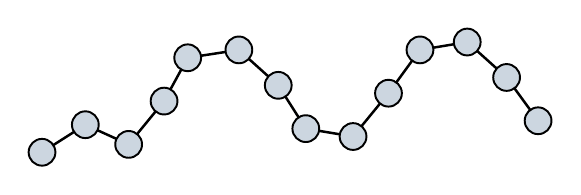
\begin{tikzpicture}
  \draw[line width=0.9pt] (0,0) -- (0.55,0.35);
  \draw[line width=0.9pt] (0.55,0.35) -- (1.1,0.1);
  \draw[line width=0.9pt] (1.1,0.1) -- (1.55,0.65);
  \draw[line width=0.9pt] (1.55,0.65) -- (1.85,1.2);
  \draw[line width=0.9pt] (1.85,1.2) -- (2.5,1.3);
  \draw[line width=0.9pt] (2.5,1.3) -- (3.0,0.85);
  \draw[line width=0.9pt] (3.0,0.85) -- (3.35,0.3);
  \draw[line width=0.9pt] (3.35,0.3) -- (3.95,0.2);
  \draw[line width=0.9pt] (3.95,0.2) -- (4.4,0.75);
  \draw[line width=0.9pt] (4.4,0.75) -- (4.8,1.3);
  \draw[line width=0.9pt] (4.8,1.3) -- (5.4,1.4);
  \draw[line width=0.9pt] (5.4,1.4) -- (5.9,0.95);
  \draw[line width=0.9pt] (5.9,0.95) -- (6.3,0.4);
  \filldraw[fill=UGblue!20,draw=black,line width=0.7pt] (0,0) circle (0.17);
  \filldraw[fill=UGblue!20,draw=black,line width=0.7pt] (0.55,0.35) circle (0.17);
  \filldraw[fill=UGblue!20,draw=black,line width=0.7pt] (1.1,0.1) circle (0.17);
  \filldraw[fill=UGblue!20,draw=black,line width=0.7pt] (1.55,0.65) circle (0.17);
  \filldraw[fill=UGblue!20,draw=black,line width=0.7pt] (1.85,1.2) circle (0.17);
  \filldraw[fill=UGblue!20,draw=black,line width=0.7pt] (2.5,1.3) circle (0.17);
  \filldraw[fill=UGblue!20,draw=black,line width=0.7pt] (3.0,0.85) circle (0.17);
  \filldraw[fill=UGblue!20,draw=black,line width=0.7pt] (3.35,0.3) circle (0.17);
  \filldraw[fill=UGblue!20,draw=black,line width=0.7pt] (3.95,0.2) circle (0.17);
  \filldraw[fill=UGblue!20,draw=black,line width=0.7pt] (4.4,0.75) circle (0.17);
  \filldraw[fill=UGblue!20,draw=black,line width=0.7pt] (4.8,1.3) circle (0.17);
  \filldraw[fill=UGblue!20,draw=black,line width=0.7pt] (5.4,1.4) circle (0.17);
  \filldraw[fill=UGblue!20,draw=black,line width=0.7pt] (5.9,0.95) circle (0.17);
  \filldraw[fill=UGblue!20,draw=black,line width=0.7pt] (6.3,0.4) circle (0.17);
\end{tikzpicture}
\end{document}
